\documentclass[11pt,reqno]{amsart}
\usepackage{pgfplots}
\usepgfplotslibrary{groupplots}
\pgfplotsset{compat=1.6}
\pgfplotsset{every axis title/.append style={at={(0.6,1.1)}}}
\usepackage{tcolorbox}
\usepackage{pgf, tikz}
\usetikzlibrary{automata, positioning, arrows, decorations.pathreplacing, decorations.pathmorphing}
\usepackage[utf8]{inputenc}
\usepackage{tikz-network}
\usepackage{amssymb}
\usepackage[utf8]{inputenc}

\begin{document}

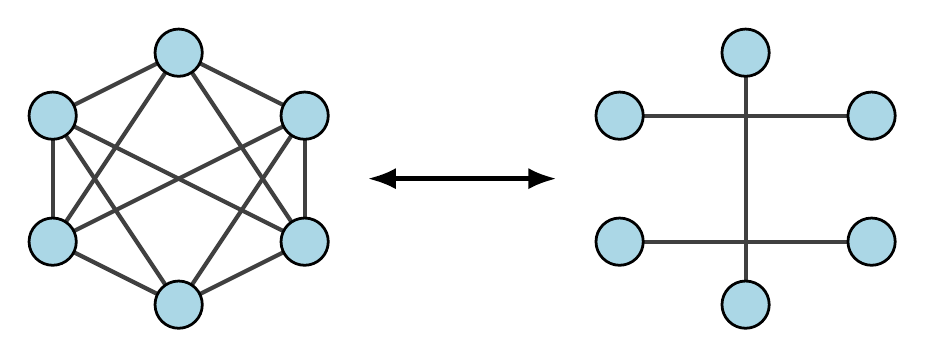
\begin{tikzpicture}[scale = 0.8]
		\Vertex[x=0,y=0]{t1}
		\Vertex[x=-2,y=1]{t2}
		\Vertex[x=-2,y=3]{t3}
		\Vertex[x=0,y=4]{t4}
		\Vertex[x=2,y=3]{t5}
		\Vertex[x=2,y=1]{t6}
		\Edge(t1)(t2)
		\Edge(t1)(t3)
		\Edge(t1)(t6)
		\Edge(t1)(t5)
		\Edge(t2)(t3)
		\Edge(t2)(t4)
		\Edge(t2)(t5)
		\Edge(t3)(t4)
		\Edge(t3)(t6)
		\Edge(t4)(t5)
		\Edge(t4)(t6)
		\Edge(t5)(t6)
		\draw[{Latex}-{Latex}, ultra thick] (3,2) -- (6,2);
		\Vertex[x=9,y=0]{p1}
		\Vertex[x=7,y=1]{p2}
		\Vertex[x=7,y=3]{p3}
		\Vertex[x=9,y=4]{p4}
		\Vertex[x=11,y=3]{p5}
		\Vertex[x=11,y=1]{p6}
		\Edge(p1)(p4)
		\Edge(p2)(p6)
		\Edge(p3)(p5)
	\end{tikzpicture}

\end{document}